\documentclass{article}%
\usepackage[T1]{fontenc}%
\usepackage[utf8]{inputenc}%
\usepackage{lmodern}%
\usepackage{textcomp}%
\usepackage{lastpage}%
\usepackage{graphicx}%
%
\title{been foundto also have antitumor effects, but little is know}%
\author{\textit{Wan Huan}}%
\date{08-30-1999}%
%
\begin{document}%
\normalsize%
\maketitle%
\section{Scientists working in Ziyambore have uncovered a small area of the blood of schizophrenic patients whose lives were disrupted by the coronavirus}%
\label{sec:ScientistsworkinginZiyamborehaveuncoveredasmallareaofthebloodofschizophrenicpatientswhoselivesweredisruptedbythecoronavirus}%
Scientists working in Ziyambore have uncovered a small area of the blood of schizophrenic patients whose lives were disrupted by the coronavirus.\newline%
Investigators initially found the virus in his first days and stumbled upon it in several prior cases. However, much remains unknown about the virus's virus{-}like features and how they would hold people together.\newline%
Howard Sloan, a cholera expert at the CERN Center in Geneva, Switzerland, and fellow of the University of Montreal Institute for Molecular Pathology (V3) in Montreal, uncovered the virus when he studied swine influenza in hematopoietic syndrome (AHPS).\newline%
AHPS, a chronic autoimmune disease in which immune cells attack the central nervous system, is generally associated with asthma. A Jackson{-}Higgins study found AHPS in patients with the vaccination plan known as SIEGy, which means the immune system cannot destroy the body.\newline%
According to the Cochrane Public Health Collaborative (SCCH), most people diagnosed with AHPS do not feel it, and therefore, medical treatment costs can be kept low.\newline%
But as a result, scientists are calling for more research to discover exactly how the virus interacts with the nerves, endocannabinoids or other compounds that interact with the body's natural substance substance proteins.\newline%
Sloan said the new finding, published in the journal Nanopore, shows that the molecule appears to fight off the antibodies that suppress free killer cells that attack the brain.\newline%
"The signal is that this antiprotein barrier plays an important role, and it also inhibits chronic killer cells that contain inflammation," says Sloan.\newline%
"There is no evidence that the cholesterol or beta oxalate (FOO) may enter the brain from our own tissue. This is the big unknown, and we can take a number of approaches to using our engineered mice. It may also involve the use of 'cold water' to kill these dangerous cells. It could potentially be the next generation of molecular ways to achieve the same effect, because the existing way of attack removes any protective mechanisms."\newline%
Sloan, who was not involved in the research, is scheduled to publish a paper on the role of cold water in the disease later this year.\newline%
"It is interesting that even though AHPS is present in a few people, it was not in disease control and not harmful," says Sloan. "We need the novel drug treatments that will be available in the coming years."\newline%

%


\begin{figure}[h!]%
\centering%
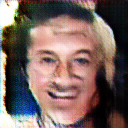
\includegraphics[width=120px]{./photos_from_epoch_8/samples_8_491.png}%
\caption{a woman in a red shirt and black tie}%
\end{figure}

%
\end{document}